Verbindet man geeignete Punkte auf zwei sich schneidenden Geraden,
dann sind die Verbindungslinien alle tangential an eine Parabel,
wie in Abbildung~\ref{30000020:figure} gezeigt.
Weisen Sie dies in den folgenden Teilaufgaben nach.
\begin{teilaufgaben}
\item
Bestimmen Sie die Gleichung einer Geraden in $\mathbb R^2$ durch die Punkte
$(t,t)$ und $(t-1,1-t)$ für $t\in\mathbb R$.
So entsteht eine Schar von Geraden mit Parameter $t$.
\item
Bestimmen Sie den Schnittpunkt der zwei Geraden mit den Werten
$t$ und $t+h$ des Parameters der Geradenschar.
\item
Bestimmen Sie den Grenzwert des Schnittpunktes für $h\to 0$.
\item
Der Grenzwert des Schnittpunktes in c) sei mit $(x,y)$ bezeichnet.
Finden Sie eine Darstellung von $y$ in der Form $y=f(x)$.
\end{teilaufgaben}

\begin{figure}[h]
\centering
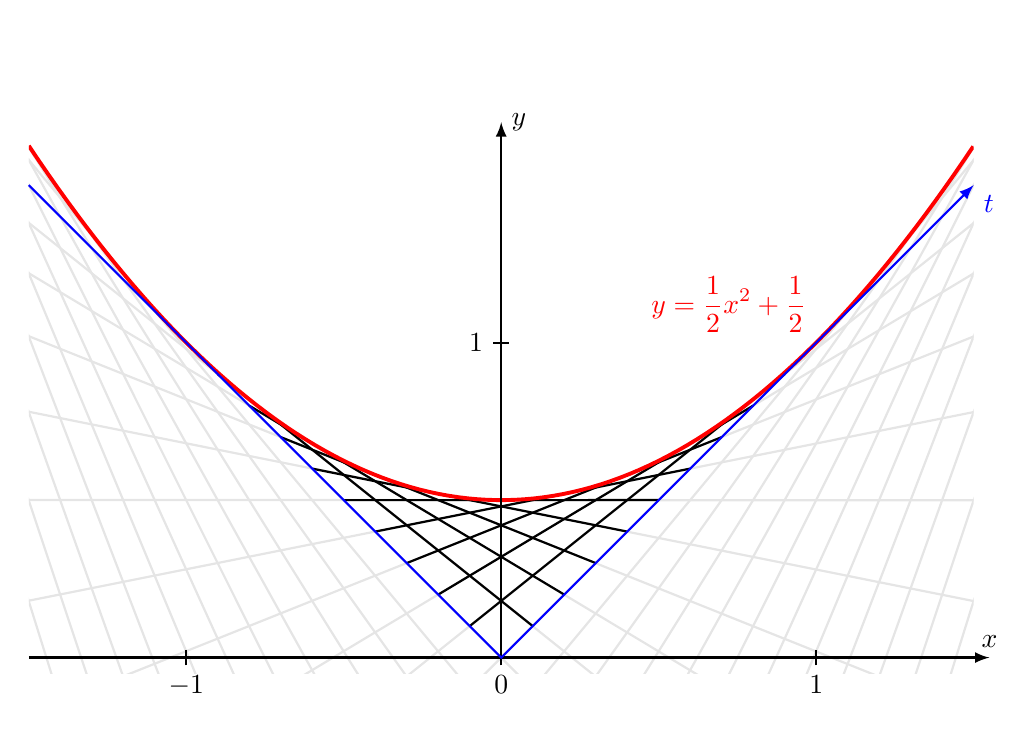
\begin{tikzpicture}[>=latex,scale=4,thick]

\begin{scope}
\clip (-1.5,-0.05) rectangle (1.5,2);
\foreach \t in {-2.5,-2.4,...,2.5}{
	% direction (1-2*\t,1)
	\draw[color=black!10]
		({-\t-2},{\t-2*(1-2*\t)})
		--
		({1-\t+2},{1-\t+2*(1-2*\t)});
}
\foreach \t in {0.1,0.2,...,0.9}{
	\draw (-\t,\t)--({1-\t},{1-\t});
}

\ifthenelse{\boolean{loesungen}}{
\node[color=red] at (1,1) [above left] {$\displaystyle y=\frac12x^2 + \frac12$};
}{}


\draw[color=red,line width=1.4pt] 
	plot[domain=-1.5:1.5,samples=100] ({\x},{0.5+0.5*\x*\x});
\end{scope}

\draw[->] (-1.5,0)--(1.55,0)  coordinate[label={$x$}];
\draw[->] (0,-0.025)--(0,1.7) coordinate[label={right:$y$}];

\draw[->,color=blue] (-1.5,1.5)--(0,0)--(1.5,1.5);
\node[color=blue] at (1.5,1.5) [below right] {$t$};

\draw (-1,-0.025)--(-1,0.025);
\node at (-1,-0.025) [below] {$-1$};
\draw (1,-0.025)--(1,0.025);
\node at (1,-0.025) [below] {$1$};
\node at (0,-0.025) [below] {$0$};
\draw (-0.025,1)--(0.025,1);
\node at (-0.025,1) [left] {$1$};

\end{tikzpicture}
\caption{Einhüllende einer Geradenschar, zu Aufgabe~\ref{30000020}.
\label{30000020:figure}}
\end{figure}

\thema{Schnittpunkt}
\thema{Geradengleichung}

\begin{loesung}
\begin{teilaufgaben}
\item
Da die Gerade durch zwei bekannte Punkte gehen muss, ist die
Parameterdarstellung der Gerade naheliegend.
Sie ist
\[
\vec{p}
=
\begin{pmatrix}t\\t\end{pmatrix}
+s
\begin{pmatrix}-1\\1-2t\end{pmatrix}.
\]
\item
Den Schnittpunkt kann man zum Beispiel mit Hilfe des Gauss-Algorithmus
finden:
\begin{align*}
\begin{tabular}{|
>{$}c<{$}
>{$}c<{$}
>{$}c<{$}
>{$}c<{$}|
>{$}c<{$}
|}
\hline
x&y&u&v&\\
\hline
1&0& 1     &  0    & t  \\
0&1&2t   -1&  0    & t  \\
1&0&  0    &  1    & t+h\\
0&1&  0    &2t+2h-1& t+h\\
\hline
\end{tabular}
&\rightarrow
\begin{tabular}{|
>{$}c<{$}
>{$}c<{$}
>{$}c<{$}
>{$}c<{$}|
>{$}c<{$}
|}
\hline
x&y&u&v&\\
\hline
 1 & 0 &  1   &  0    & t  \\
 0 & 1 & 2t-1 &  0    & t  \\
 0 & 0 & -1   &  1    & h  \\
 0 & 0 & 1-2t &2t+2h-1& h  \\
\hline
\end{tabular}
\\
\rightarrow
\begin{tabular}{|
>{$}c<{$}
>{$}c<{$}
>{$}c<{$}
>{$}c<{$}|
>{$}c<{$}
|}
\hline
x&y&u&v&\\
\hline
 1 & 0 &  1   &  0    &  t      \\
 0 & 1 & 2t-1 &  0    &  t      \\
 0 & 0 &  1   & -1    & -h      \\
 0 & 0 &  0   &  2h   & h+2h(1-2t) \\
\hline
\end{tabular}
&\rightarrow
\begin{tabular}{|
>{$}c<{$}
>{$}c<{$}
>{$}c<{$}
>{$}c<{$}|
>{$}c<{$}
|}
\hline
x&y&u&v&\\
\hline
 1 & 0 &  1   &  0    &   t   \\
 0 & 1 & 2t-1 &  0    &   t   \\
 0 & 0 &  1   &  0    & t-h+1 \\
 0 & 0 &  0   &  1    &   1-t \\
\hline
\end{tabular}
\\
\rightarrow
\begin{tabular}{|
>{$}c<{$}
>{$}c<{$}
>{$}c<{$}
>{$}c<{$}|
>{$}c<{$}
|}
\hline
x&y&u&v&\\
\hline
 1 & 0 &  1   &  0    &   t   \\
 0 & 1 & 2t-1 &  0    &   t   \\
 0 & 0 &  1   &  0    & 1-t-h \\
 0 & 0 &  0   &  1    & 1-t   \\
\hline
\end{tabular}
&\rightarrow
\begin{tabular}{|
>{$}c<{$}
>{$}c<{$}
>{$}c<{$}
>{$}c<{$}|
>{$}c<{$}
|}
\hline
x&y&u&v&\\
\hline
 1 & 0 &  0   &  0    & 2t+h-1 \\
 0 & 1 &  0   &  0    &2t^2+2ht-2t-h+1\\
 0 & 0 &  1   &  0    & 1-t-h \\
 0 & 0 &  0   &  1    &   1-t \\
\hline
\end{tabular}
\end{align*}
Daraus lesen wir ab, dass der Schnittpunkt $(2t+h-1, 2t^2+2ht-2t-h+1)$ ist.
\item
Der Grenzwert ist
\[
\left.
\begin{aligned}
\lim_{h\to 0} x(h) &=\lim_{h\to 0} (2t+h-1) = 2t-1
\\
\lim_{h\to 0} y(h) &=\lim_{h\to 0} (2t^2+2ht-2t-h+1) = 2t^2-2t+1
\end{aligned}
\quad
\right\}
\quad\Rightarrow\quad
\lim_{h\to 0} S = (2t-1, 2t^2-2t+1).
\]
\item
Das Quadrat $x^2=(2t-1)^2=4t^2-4t+1$ von $x=2t-1$ sieht sehr ähnlich aus wie
$y=2t^2-2t+1$.
Den führenden Koeffizienten kann mit einem Faktor $\frac12$ in Übereinstimmung
bringen: $\frac12x^2 = 2t^2-2t+\frac12$, dann fehlt aber noch ein
konstanter Summand der Grösse $\frac12$.
So bekommen wir
\[
y=\frac12x^2 +\frac12,
\]
dies ist die in Abbildung~\ref{30000020:figure} rot eingezeichnete Parabel.
\end{teilaufgaben}
Alternativ kann man statt eines $4\times 4$-Gleichungssystems die beiden
Paramterdarstellungen auch gleichsetzen:
\begin{align*}
\begin{pmatrix}t\\t\end{pmatrix}
+r_1\begin{pmatrix}-1\\1-2t\end{pmatrix}
&=
\begin{pmatrix}t+h\\t+h\end{pmatrix}
+r_2\begin{pmatrix}-1\\1-2t-2h\end{pmatrix}
\\
r_1\begin{pmatrix}-1\\1-2t\end{pmatrix}
-r_2\begin{pmatrix}-1\\1-2t-2h\end{pmatrix}
=
\underbrace{
\begin{pmatrix}
-1&1\\
1-2t&-1+2t+2h
\end{pmatrix}
}_{\displaystyle=A}
\begin{pmatrix}r_1\\r_2 \end{pmatrix}
&=
\begin{pmatrix}h\\h\end{pmatrix}.
\end{align*}
Dieses Gleichungssystem kann man mit Hilfe der inversen Matrix $A^{-1}$
auflösen:
\begin{align*}
A^{-1}
&=
\frac1h
\begin{pmatrix}
-t-h+\frac12 & \frac12 \\
-t+\frac12 & \frac12
\end{pmatrix}
&&\Rightarrow&
\begin{pmatrix}r_1\\r_2\end{pmatrix}
=
A^{-1}\begin{pmatrix}h\\h\end{pmatrix}
=
\begin{pmatrix}
1-t-h\\
1-t
\end{pmatrix}.
\end{align*}
Jetzt kann man $r_2=1-t$ in die Geradengleichung einsetzen und erhält
\begin{align*}
\begin{pmatrix}x\\y \end{pmatrix}
&=
\begin{pmatrix}t+h\\t+h\end{pmatrix}
+(1-t)
\begin{pmatrix}-1\\1-2t-2h\end{pmatrix}
=
\begin{pmatrix}
2t+h-1\\
2t^2+2ht-2t-h+1
\end{pmatrix}
\end{align*}
Dies ist der gleiche Schnittpunkt wie mit dem Gauss-Tableau gefunden.
(Lösung von Rolf Camathias.)
\qedhere
\end{loesung}

\begin{bewertung}
Geradengleichung Stützvektor ({\bf P$_0$}) und Richtungsvektor ({\bf R})
je ein Punkt,
Tableau ({\bf T}) 1 Punkt, Schnittpunkt ({\bf S}) 1 Punkt,
Grenzwert ({\bf G}) 1 Punkt,
Funktionsgleichung ({\bf F}) 1 Punkt.
\end{bewertung}

